\documentclass[a4paper,12pt,twoside]{article}
\usepackage{Omdtz}

%I will design the first page later
\begin{document}
  \begin{tikzpicture}[remember picture, overlay]
  \node[opacity=0.3,inner sep=0pt] at (current page.center)
   {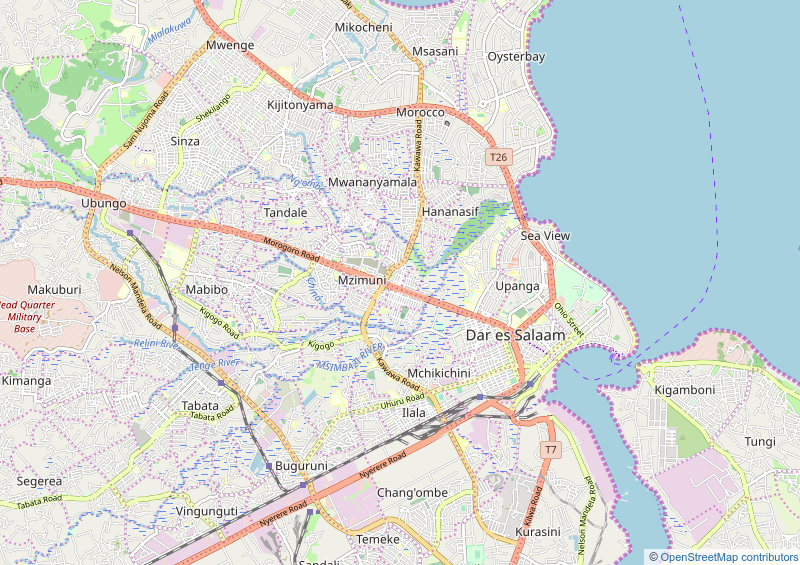
\includegraphics[width=\textwidth,height=\textheight]{Images/OSM.png}};%i will change the image later
  \end{tikzpicture}
  

\begin{center}
\vspace{5cm}
\Huge \color{OMDTZblue} \textbf {OpenMap Development Tanzania} 

\textbf{Organization Profile} 
    
\end{center}
\newpage

% Reduce the spacing between Table of Contents items to get it down to 1 page
\newpage
\renewcommand{\baselinestretch}{1.3}\normalsize
\tableofcontents
\renewcommand{\baselinestretch}{1.0}\normalsize

\newpage
\section{About the Organization}
%\label{abouttheorganization}

OpenMap Development Tanzania (OMDTZ) is a registered NGO based in Dar es Salaam and operating across Tanzania. Since its establishment in 2017, OMDTZ has promoted a number of community mapping projects, generated map awareness, actively pledged open data sets and continued to build a network of enthusiastic mappers in Tanzania. 

Similar to the Humanitarian OpenStreetMap Team (https://www.hotosm.org/), all activities are set up around the global OpenStreetMap (OSM - https://www.openstreetmap.org/) project, which is both a map and database of geographic data owned by the contributors themselves: anyone is able to view, create and use this information for free. 

OMDTZ staff have been heavily involved in the success of community mapping projects in Tanzania through engaging and training community members to, for instance, map the flood-prone areas of Dar es Salaam for flood resilience purposes under the Ramani Huria project (a World Bank and DFID funded project) and mapping the Bukoba region to strengthen response and preparedness to disasters in this earthquake-affected area. 

We also involve people with different backgrounds ranging from technology, social, economic, political, academic and community members who are the centre of our operations.



\subsubsection {Vision}
Organization’s mission is to have a vibrant Tanzanian community which is united, organised, growing to assist and get involved in national and global development goals via mapping.


\subsubsection{Mission}
The organization is on a mission to promote open data and open source and applying these principles to assist organizations and individuals in local and international settings to manage and solve social, economic and community challenges through mapping.

\subsubsection{Objectives}

General Objective
………………………………………………………………….
………………………………………………………..(Innocent)


Specific Objectives
\begin{itemize}

\item To raise awareness on the community on mapping and maps throughout Tanzania
\item To enable training and capacity building that will enable individuals and organization to manage social economic and community challenges
\item To enable the creation of opportunities for members of the community to engage in global sustainable development initiatives.
\item To promote innovations from community members that will provide solutions to challenges in their communities for social and economic development
\item To take part and facilitate mapping initiatives in a local and global community.
\item To provide education to the community on OpenStreetMap and open data.
\item To empower the community on cartographic tools and skills to business, universities, government agencies and different organization.
\end{itemize}

\newpage
\section{Approach and Strategy}
%\label{approachandstrategy}

OMDTZ considers the following principles when implementing different activities--ranging from design of activities to field operations

\textbf{Participatory approach (partners)}: we encourage our beneficiaries especially community member in the project area of interest to participate actively in our programmes right from needs assessment to implementation, monitoring and evaluation, and benefit-sharing(data sharing) through workshops and meetings prepared

\textbf{People-centred approaches}: involving community members, and making the community a centre of our approach.

\textbf{Coordination and collaboration}: our activities will effectively be coordinated with the government, and non-governmental organizations including institutions where necessary, starting from a grassroots level ie Shina, sub ward, ward, district, region/city and the central government depending on the hierarchy needed for specific projects.

\textbf{Transparency}: all the program activities and corresponding budget allocated for that particular place are transparent; anyone at any time can have access to this information (if requested). Our data will also be shared freely unless otherwise stated in some specific data sets (i.e sensitive datasets)

\textbf{Focus on the demand}: Projects will be designed and implemented according to the needs of the beneficiaries.--Projects will not be imposed from the top.

\newpage
\section{Core Values}
%\label{corevalues}
\begin{itemize}

\item \textbf{Gender consideration:} OMDTZ considers gender norms, roles and relations for women and men and how they affect access to and control over resources; considers women and men's specific needs and might intentionally target and benefit specific groups of women or men to achieve certain policy or programme goals or meet certain needs.

\item \textbf{Human right:} Guided through its humanitarian policies principles of human rights which actively nurture all aspect of human rights and integrates it to enable and empower the people for asserts their fundamental right.

\item \textbf{Data sharing:}  OMDTZ  will share data openly with multiple users unless otherwise stated in case there are specific data sets that need protection then the procedures of sharing and use of these type of data will be clearly described

\item\textbf{Clean funds:}  OMDTZ shall only receive clean funds that are not connected with any illegal or intentions that do not comply with organizations principles

\item\textbf{Child rights:} Observing national and international children rights i.e no child labour etc

\item \textbf{Religious freedom:} "Everyone has the right of freedom of thought, conscience and religion; this right includes freedom to change his religion or belief, and freedom, either alone or in community with others and in public or private, to manifest his religion or belief in teaching, practice, worship and observance." (Universal Declaration of Human Rights, Article 18)

\item\textbf{Fund Raising: }OMDTZ as a recipient of such funds, it should be open and transparent, be accountable to the donor, use the funds responsibly and according to the intent of the donor, and allow the funding individuals and organizations to be able to have insight into the project at all times. Fundraising activity also must be consistent with the mission of the NGO.
\end{itemize}

\newpage
\section{Organization Policies}
%\label{policies}

OMDTZ is guided by the following policy (Note; Each policy must also abide by governments’ policies and laws.

\textbf{Finance Policy:} OpenMap Development Tanzania uses the accrual basis of accounting. The accrual basis is the method of accounting whereby revenue and expenses are identified with specific periods of time, such as a month or year, and are recorded as incurred.  This method of recording revenue and expenses is without regard to the date of receipt or payment of cash.

\textbf{Human Resources Policy:} The organisation promotes the importance of HR policies and strategies, particularly those relating to work relationships and acceptance of diversity, to all levels of the organisation. To ensure the quality of work relationships, staff well being, organisational justice, openness to diversity and emotional climate.

\textbf{Security Policy:}.......... ......................................................................................................................

\textbf{Technical and Innovation policy:}
......................................................................................

\textbf{Public Relations and Communications Policy:} Considerable importance on effective communication among one another regardless of position on the organization, race, religion, gender etc. This policy guides all communications internally and externally. All employees are to adhere to the policy and failure to do so may result in disciplinary actions basing on the constitution of OMDTZ.

\textbf{Data Policy}     .......................................................................

\textbf{Procurement Policy}       .........................................................................................................................

\newpage
\section{Projects and Experience}
%\label{projectsandexperience}

Ramani Huria

Ramani Huria is a community-based mapping project that began 2015 in Dar es Salaam, Tanzania, training university students and local community members to create highly accurate maps of the most flood-prone areas of the city. As the maps have taken shape – their benefits have multiplied and their potential magnified, now serving as foundational tools for development within all socio-economic spheres beyond flood resilience. The project is supported by funding from the UK Department for International Development through the Tanzania Urban Resilience Programme. OMDTZ works on providing survey information together with our affiliate HOT.


Data Zetu

Data Zetu (“Our Data” in Swahili) aims to empower communities to make better, more evidence-based decisions to improve their lives. The program works with communities across Tanzania to discover issues that matter most to them. Then we work with stakeholders to arm them with skills and tools to make sense of data related to those challenges. As a result, we’re helping to foster the use of open data that is relevant, hyperlocal, and actionable.

OMDTZ participated again as a HOT affiliate to support in providing Geospatial data and visualizations --that provide evidence to the challenges pointed by community members--ie making maps on time is taken by women to reach maternity health care and visualize it on a map. 

Mini-Grids Rural electrification

In partnership with the International Finance Corporation (IFC), and input from related projects executed by RLI and INTEGRATION, the Humanitarian OpenStreetMap Team (HOT) through OMDTZ in Tanzania implemented this project - a data collection initiative to help inform rural electrification plans in Tanzania. In just two months, a team of remote digitizers managed to add over 4,000,000 buildings to the map, whilst the field team collected data across 2000 settlements. This data will be used to improve access to electricity in Tanzania, propelling development initiatives in rural areas.  

Innovation Ecosystem Mapping

This is the first stand-alone project for OMDTZ, The project involves maintenance of an online platform for innovation ecosystem map in Tanzania. The online interactive map will show vast information about the innovators in the country. We are focusing on administering and managing the innovation map as a platform to bridge the gap and provide a conducive environment and linkages among innovation stakeholders in the country. The end goal is to build the map into a sustainable platform to support the Innovation Ecosystem of Tanzania. 
5. Aerial Riparian Solid Waste mapping

This project had the focus to get aerial images to analyse river banking to get the trash data alongside rivers for that could help decision-makers. This project for the aerial data collection intended to get the data alongside major rivers that are drains their water to the Indian Ocean, these rivers that were targeted are Msimbazi, Mpiji, Tegeta, Mzinga, and Kizinga.

%\newpage
\subsubsection{Major Projects Summary}

\begin{center}

\begin{tabular}{|c|c|c|c|c|c|}
\hline
 \bfseries SN & \bfseries Project Name & \bfseries Location & \bfseries Affiliates/Partners & \bfseries Donor/Funder & \bfseries Year(s) \\
 \hline
1&  Ramani Huria & Dar es Salaam & - & World Bank & 2015 to 2019 \\
\hline
2 & Data Zetu & Dar es Salaam & {} & {} & {}\\
{}&{}& and Mbeya & - & PEPFAR/MCC & 2017-2018 \\
\hline
3 & Mini-Grids & {}& {} &{} &{}\\ 
{} & Rural & Tanzania & - & IFC & 2017-2018\\
{} & Electrification & {} & {} & {} & {}\\ 
\hline
4 & Innovation & {} & {} & {} &{} \\ 
{} & Ecosystem & Tanzania & - & HDIF & 2018-2020\\ 
{} & Mapping & {} & {} & {} &{}\\
\hline
5 & Aerial & {} &{} &{} &{}\\
{} & Riparian & {} & {} & {} & {}\\ 
{} & Solid Waste  & Dar es salaam & Nipe Fagio & Palladium & 2019\\
{} & Mapping & {} &{} & {} &{}\\
\hline
\end{tabular}
\end{center}

\end{document}
